\documentclass[twocolumn]{aastex61}
\pdfoutput=1 
\usepackage{upgreek}
\usepackage{color} 
\usepackage{amsmath}
\usepackage{graphicx}
\usepackage{subfigure}
\usepackage{algorithm,algorithmic}
\usepackage{mathrsfs}

\usepackage{amssymb}

\usepackage{graphicx}
\usepackage{float}
%\usepackage{caption}
%\usepackage{subcaption}
\usepackage{natbib}
\usepackage{footnote}

\usepackage{bbold}

%\usepackage{deluxetable}
%\usepackage{morefloats}

%\usepackage{amssymb}
%\usepackage{amsmath}
%\usepackage{epstopdf}
%\usepackage{color}

%\usepackage{mathrsfs}

\def \frb {FRB Search Algorithm}
\def \halpha {\ensuremath{\mathrm{H\alpha}}}
\def \hbeta {\ensuremath{\mathrm{H\beta}}}


\newcommand{\be}{\begin{eqnarray}}
\newcommand{\ee}{\end{eqnarray}}
\newcommand{\etal}{et al.}


\newcommand{\Halpha}{\rm H\alpha}
\newcommand{\EM}{{\rm EM}}
\newcommand{\DM}{{\rm DM}}
\newcommand{\SM}{{\rm SM}}
\newcommand{\SFR}{\ensuremath{\mathrm{SFR}}}

\newcommand{\DMhatzero}{\rm \widehat{\DM}}
\newcommand{\DMhatFRB}{\rm \widehat{\DM}({\rm FRB})}

\newcommand{\Ss}{S({\rm\halpha})_{\rm s}}
\newcommand{\EMs}{{\rm EM}_{\rm s}}
\newcommand{\EMsHalpha}{{\rm EM}(\halpha)_{\rm s}}
\newcommand{\EMsHbeta}{{\rm EM}(\hbeta)_{\rm s}}
\newcommand{\DMsHalpha}{{\rm DM}(\halpha)_{\rm s}}
\newcommand{\DMs}{\widehat{\rm DM}_{\rm s}}


\newcommand{\EMDM}{{\rm EM_{\rm DM}}}
\newcommand{\EMSM}{{\rm EM_{\rm SM}}}

\turnoffedit

\begin{document}

%\setlength{\fboxsep}{0pt}%
%\setlength{\fboxrule}{0.5pt}%

%\received{\today}
\revised{\today}
%\accepted{\today}
%\submitjournal{ApJ}

\shorttitle{2D-FFT search Algorithm }
\shortauthors{C.H.Niu~et al.}

\title{Using 2D-FFT to search Fast Radio Burst}%\footnote{peterniu@nao.cas.cn}}


%\correspondingauthor{Xuelei~Chen}
\email{}

\author{C.H. Niu}
\affil{Central China Normal University \\
Luoyu Road,Wuhan, China}
\affil{National Astronomy Observatory , Chinese Academy of Sciences \\
Datun(A) Road,No.30,Beijing, China}
\affil{University of California Berkeley, Campbell Hall 339, Berkeley CA 94720}

\author{Y.C. Li}
\affil{National Astronomy Observatory , Chinese Academy of Sciences \\
Datun(A) Road,No.30,Beijing, China}
\author{S.F. Zuo}
\affil{National Astronomy Observatory , Chinese Academy of Sciences \\
Datun(A) Road,No.30,Beijing, China}

\author{F.Q. Wu}
\affil{National Astronomy Observatory , Chinese Academy of Sciences \\
Datun(A) Road,No.30,Beijing, China}

\author{Ue-li Pen}
\affil{CITA}
\affil{National Astronomy Observatory , Chinese Academy of Sciences \\
Datun(A) Road,No.30,Beijing, China}

\author{X.L. Chen}
\affil{National Astronomy Observatory , Chinese Academy of Sciences \\
Datun(A) Road,No.30,Beijing, China}







\begin{abstract}

Fast Radio Burst have been found from pulsar data for many years. There are several FRB search algorithm like tree algorithm, FDMT et. Here we proposed a different FRB searching algorithm which basically trace a curve in frequency-time image. This algorithm is mainly realized by two dimensional Fast Fourier Transform. We take a 2D FFT on the $f^{-2}(t)$ data map, Then trace the signal along the angle of straight line. In this searching method, it's easier to remove RFI in large scale and will bring a speed up benefit in well-developed 2D FFT library both in CPU and GPU code. \\


Fast Radio Burst is a high energy radio signal found in the Universe. The first one is found by Lorimer Duncn in 2007, now people always call it as Lormeter burst. Like Pulsar, It’s a wide band radio sginal, when it go through the inter stellar or inter galaxy medium, the higher frequency will go faster than lower frequency. When Signal go through dense of ISM  The origin of FRB is still unclear, there are lots of theories trying to describe what FRB is.  \\






% We discuss the implications of the first FRB host being a low-metallicity dwarf galaxy for source models, future searches for FRB hosts, and FRB rates.

\end{abstract}

\keywords{2DFFT ,FAST radio burst }

\section{Introduction}
 \label{sec:intro}
Fast radio bursts (FRBs) are bright ($\sim$Jy) and short ($\sim$ms) bursts of radio emission that have dispersion measures (DMs) in excess of the line of sight DM contribution expected from the electron distribution of our Galaxy. To date 18 FRBs have been reported
%\footnote{\url{http://www.astronomy.swin.edu.au/pulsar/frbcat/}} \citep{pbj+16}
 --- most of them detected at the Parkes telescope \citep{lbm+07,tsb+13,bb14,kskl12,rsj15,pbb+15,kjb+16,cpk+16,rsb+16} and one each at the Arecibo \citep{sch+14} and Green Bank telescopes \citep{mls+15}. 

A plethora of source models have been proposed to explain the properties of FRBs \citep[see e.g.][for a brief review]{katz16}. According to the models, the excess DM for FRBs may be intrinsic to the source, placing it within the Galaxy; it may arise mostly from the intergalactic medium, placing a source of FRBs at cosmological distances ($z\sim0.2-1$) or it may arise from the host galaxy, placing a source of FRBs at extragalactic, but not necessarily cosmological, distances ($\sim100$\,Mpc).

Since the only evidence to claim an extragalactic origin for FRBs has been the anomalously high DM, some models also attempted to explain the excess DM as a part of the model, thus allowing FRBs to be Galactic. All FRBs observed to date have been detected with single dish radio telescopes, for which the localization is of order arcminutes, insufficient to obtain an unambiguous association with any object. To date, no independent information about their redshift, environment, and source could be obtained due to the lack of an accurate localization of FRBs. \citet{kjb+16} attempted to identify the host of FRB\,150418 on the basis of a fading radio source in the field that was localized to a $z=0.492$ galaxy. However, later work identified the radio source as a variable active galactic nucleus (AGN) that may not be related to the source \citep{wb16,bbt+16,gmg+16,jkb+16}.

%\subsection{Interferometric Localization of \frb}
 Repeated radio bursts were observed from the location of the Arecibo-detected \frb\ \citep{ssh+16a,ssh+16b}, with the same DM as the first detection, indicating a common source. As discussed by \citet{ssh+16a}, it is unclear whether the repetition makes \frb\ unique among known FRBs, or whether radio telescopes other than Arecibo lack the sensitivity to readily detect repeat bursts from other known FRBs.

\citet{clw+16} used the Karl G. Jansky Very Large Array (VLA) to directly localize the repeated bursts from \frb\ with 100-mas precision and reported an unresolved, persistent radio source and an extended optical counterpart at the location with a chance coincidence probability of $\approx 3\times10^{-4}$ --- the first unambiguous identification of multi-wavelength counterparts to FRBs. Independently, \citet{mph+16} used the European VLBI Network (EVN) to localize the bursts and the persistent source and showed that both are co-located within $\sim12$ milliarcseconds.

Here we report a new algorithm to search FRBs . 

%In Section~\ref{sec:obs}, we discuss the observations and data analysis. In Section~\ref{sec:results}, we identify the counterpart as the host galaxy of the FRB and present its redshift and spectral characteristics. In Section~\ref{sec:discussion}, we discuss the physical properties of the environment and the implications for source models for FRBs.

%Constraining the multitude of FRB models is complicated by the difficulty in localizing FRBs, as all have been found in beams of single dish radio telescopes, which are several arcminutes in diameter. Realtime detection and rapid multi-wavelength follow-up have so far been unsuccessful \citep{pbb+15,kjb+16}.

%\textit{Paragraph on repeating FRB 121102 and VLA localization.}


\section{Basics of Incoherent Dedispersion}
\label{sec:obs}

The dispersion of the electromagnaetic wave pulse cause a delay in arrival time at frequency $\nu$ compared with the reference frequency $\nu_0$, which is given by :
\begin{equation}
\Delta t (\nu) = -D(\nu^{-2} -\nu^{-2}_{0})\label{eq:Disperse relation}
\end{equation}
where D is the dispersion measure times a dispersion constant. Thus , We may model a burst with a very short intrinsic width as :
\begin{equation}
I(t,\nu)=I_0(\nu)\delta_D(t-t_s -\frac{D}{\nu^2})  
\end{equation}
Where $\delta D$ is the Dirac delta function, $t_s$ marks the signal starting time for infinitely high frequency. If the bandwidth is small, we can approximate
\begin{equation*}
\frac{D}{\nu^{2}}\approx\frac{D}{\nu_0^2}(1-2\frac{\nu-\nu_0}{\nu_0})
\end{equation*}
denote $\Delta \nu \equiv \nu - \nu_0$, and assume that the spectrum is not too steep such that within the observing band the signal is constant, then
\begin{equation}
\begin{aligned}
I(t,\nu) & \approx I_0\delta_D(t-t_s-\frac{D}{\nu_0^2}(1-2\frac{\Delta\nu}{\nu_0}) ) \\
		 & = I_0\delta_D(t -t_0 +\frac{2D}{\nu_0^3}\Delta\nu)
\end{aligned} 
\end{equation} \label{eq:linear assumpution}
where $t_0$ is the arrival time of the signal at thre reference frequency $\nu_0$. \\
	Now consider an integral of this signal between frequency $\nu_1 $ and $\nu_2$ , the signal strength would be
\begin{equation}
s = \int d \nu \int dtI(t,\nu)=(\nu_2 -\nu_1)I_0 = I_0B
\end{equation}
Where $B =\nu_2 -\nu_1$ is the bandwidth. Now consider the noise. Suppose the data is digitized with time interval $\delta t$ and frequency channel bandwidth $\delta \nu$. For the incoherent dedispersion, the signal within each time interval and frequency channel is 
\begin{equation}
I_n = \frac{2k T_{sys}}{A_{\rm eff} \sqrt{\delta \nu \delta t}} 
\end{equation}
Suppose we are observing between $\nu_1$,$\nu_2$ with a total of $N_\nu$ channels, and processing a time interval $T = N_t \delta t$ where $T \geq \Delta t(\nu_1) -\Delta t(\nu_2)$, i.e. the whole of the dispersed signal is within the data frame. \\
	For incoherent dedispersion , in the absence of the pulse signal, the whole read out of the data frame is given by 
	\begin{equation}
	\begin{aligned}
	n &=  \int d\nu\int dt I_n = \frac{2kT_{sys}}{A_{\rm eff}}\frac{(\nu_2 -\nu_1) T}{\sqrt{\delta \nu \delta t}} \\
	  &=  \frac{2kT_{sys}}{A_{\rm eff}} B^{1/2} T^{1/2}N_{\nu}^{1/2}N_t^{1/2}
	\end{aligned}
	\end{equation}
So the raw signal to noise ratio is given 
\begin{equation}
{\rm SNR}_{raw} = \frac{I_0 A_{\rm eff}}{2kT_{sys}}\left(\frac{B}{N_\nu N_t T}\right)^{1/2}
\end{equation}

	 In a perfect incoherent dedispersion , we sum up all the signal, which is still given by $s$. However, we compare it with the noise in the same dedispersion $\nu -t $ track, not the whole data frame. The noise along the same track is given by 
	 \begin{equation}
	 n = \int d\nu \int dt I_n \delta _D(t- t_0 + \frac{2D}{\nu_0 ^3}\Delta \nu)=BI_n
	 \end{equation}
Then 
\begin{equation}
{\rm SNR} _{opt} = \frac{I_0}{I_N}=\frac{I_0 A_{\rm eff}}{2kT_{sys}} \left( \frac{BT}{N_{\nu} N_t} \right)^{1/2}
\end{equation}

Now consider a pulse of finite width. We replace the Dirac $\delta$ function by a Gaussian function with the same normalization
\begin{equation}
\delta _D(t-t') \to g(t-t') \equiv \frac{1}{(2\pi)^{1/2} \sigma} \exp[-\frac{(t-t')^2}{2\sigma^2_t}]
\end{equation}
If the pulse intrinsic width $\sigma > \delta t$, then in a dedispersion along the track only the part of the signal within one time bin would be included, which gives
\begin{equation}
\int^{+\delta t}_{-\delta t} d \Delta t\frac{1}{\sqrt{2\pi }\sigma}e^{-\Delta t^2 /2\sigma^2}=erf(\frac{\delta t}{\sqrt{2}\sigma})\approx\sqrt{\frac{2}{\pi}}\frac{\delta t}{\sigma}
\end{equation}
Where the last holds for the case $\delta t \ll \sigma$, so in this case
\begin{equation}
s =I_0B\sqrt{\frac{2}{\pi}}\frac{\delta t}{\sigma}
\end{equation}
While the noise is still given by Eq.(8), so in this case
\begin{equation}
{\rm SNR}_{fin} = \frac{I_0}{I_n}=\frac{I_0A_{\rm eff}}{2kT_{sys}}\left( \frac{BT}{N_t N_{\nu}} \right) ^{1/2} \sqrt{\frac{2}{\pi}}\frac{\delta t}{\sigma}
\end{equation}
\\ \\


%\section{Intensity after 2D FFT}
%\label{sec:results}
%The usual Fourier transform is :
%\begin{equation}
%\begin{aligned}
%\widetilde{f}(\omega) & =\frac{1}{2\pi} \int f(t)e^{-i\omega t}dt \\
% f(t) & = \int \widetilde{f}(\omega)e^{i\omega t}d\omega
% \end{aligned}
%\end{equation}
%For$ f(t) = \delta _D(t-t_0), \widetilde{\omega} = \frac{1}{2\pi}e^{-i\omega t_0}$. Using the relation :
%\begin{equation}
%\int d\omega e^{i\omega t_0} = 2\pi \delta _D (t_0)
%\end{equation}
%we find the above indeed form a Fourier pair. However , here we want to use $\nu$ instead of $\omega$, then the Fourier transform pair are:
%\begin{equation}
%\begin{aligned}
%\widetilde{f} (\nu) &= \frac{1}{2\pi}\int f(t) e^{-i2\pi \nu t}dt \\
%f(t) &= 2\pi \int \widetilde{f}(\nu) e^{i2\pi \nu t} d\nu
%\end{aligned}
%\end{equation}
%\underline{ The 2D transform of the signal $I(\nu,t)$ is} 
%\begin{equation}
%\widetilde{I}(f,\tau)=\int d\nu~e^{-2\pi i \nu \tau} \int dt~e^{-2\pi ift}I(t,\nu)
%\end{equation}
%where we denote the Fourier conjugate variable of $\nu,t$ as $\tau,f$ to avoid confusion. For the pulse signal given by Eq.(2),
%\begin{equation}
%\begin{aligned}
%\widetilde{I}(f,\tau) &= \int d\nu e^{-2\pi i\nu \tau}I_0 e^{-2\pi i f(t_0 - \frac{2D}{\nu ^3 _0}\Delta \nu)} \\								
%								&= I_0 e^{-i2\pi f(t_0 + \frac{2D}{\nu ^2 _0})} 
%								\delta_D (\tau - \frac{2Df}{\nu ^3 _0})
%\end{aligned}
%\end{equation} 
%Note $\widetilde{I}(\tau,f)$ is non-zero only on the staight line $\tau - \frac{2Df}{\nu ^2 _0}=0$, and the value is a complex number whose phase angle gives the arrival time. For the pulse with finite width,
%\begin{equation}
%\widetilde{I}(f,\tau) = \int d\nu e^{-2\pi i \nu \tau}\int dt~e^{-2\pi ift}\cdot I_0 \frac{1}{\sqrt{2\pi}\sigma}e^{-\frac{(t-t')^2}{2\sigma ^2}}
%\end{equation}
%where $t'=t_0 - \frac{2D}{\nu _0 ^3}\Delta \nu$.  Thus we could get signal intensity with finite width $\sigma$ after 2D FFT is:
%\begin{equation}
%\begin{aligned}
%\widetilde{I}(f,\tau)  & = \int d\nu~ e^{-2\pi i\nu \tau}I_0  e^{-i2\pi ft'}e^{-\frac{(2\pi f\sigma)^2}{2}} \\
%%&= I_0e^{-i2\pi f(t_0 + \frac{2D}{\nu _0 ^2})}e^{-\frac{(2\pi f\sigma)^2}{2}}\int d\nu~exp[-i2\pi\nu(\tau - \frac{2Df}{\nu ^3_0})] \\
%&= {I_0} e^{-i2\pi f(t_0+\frac{2D}{\nu ^2 _0})}e^{-\frac{(2\pi f\sigma)^2}{2}}\delta _D (\tau - \frac{2Df}{\nu ^3 _0})
%\end{aligned}
%\end{equation}
%Note this is similar to Eq(18) except for the factor $e^{-\frac{(2\pi f \sigma)^2}{2}}$,  {\color{red}this limits the usable range of f to $|f.|<(2\pi\sigma)^{-1}$. }
%\\ \\
%%%%%%%%%%%%%%%%%%%
%\subsection{Transform to polar coordinates}
%\label{sec:discussion}
%We can take $\frac{2f}{\nu _0 ^3},\tau$ as the $x,y$ in Cartesian coordinates, then the polar coordinates $\rho,\theta$ can be defined as 
%\begin{equation}
%\begin{aligned}
%\rho ^2 &= \left(\frac{2f}{\nu _0 ^2}\right) ^2 + \tau ^2 \\
%\tan\theta &= \frac{\tau}{2f/\nu ^2 _0} 
%\end{aligned}
%\end{equation}
%with $\tan \theta = -D$ for the track satisfy Eq.(20). Conversely, 
%\begin{equation}
%\begin{aligned}
%f &= \frac{\nu ^2 _0}{2}\rho \cos\theta \\
%\tau &= \rho \sin \theta
%\end{aligned}
%\end{equation}
%Then 
%\begin{equation}
%\begin{aligned}
%\widetilde{I}(\rho, \theta) = ~&\frac{I_0}{2\pi}e^{-i2\pi\left(\frac{\nu ^2 _0\cdot t}{2}-D \right)\rho\cos\theta}~\\ 
%\cdot & ~e^{-\frac{\pi^2\sigma ^2 \nu _0 ^4}{2}\rho ^2 \cos ^2 \theta}\rho ^{-1} \delta _D (\theta + \arctan D)
%\end{aligned}
%\end{equation}
%%%%%%%%%%%%%%%%%%

\section{Implemented 2DFFT on burst search}
Assuming data output from Transient Incoherent Search backend are in $(f,t)$ format with size $[N_{ch},N_{tsamp}]$. We could get the signal line are showing up as a curve line which are complied with relationship of $f^{-2}\sim t$ in raw data map from eq. (\ref{eq:Disperse relation}). As the form of curve after 2D-FFT is much more complex than a straight line. Hence we take the 2D-FFT on $(f^{-2},t)$ map. In order to get $(f^{-2},t)$ map, we use interpolation along the frequency axis in $(f,t)$ map. The total pixel number of $(f^{-2},t)$ map keep same, so that total information could get conservation. In this case, re-bin data still has shape of $[N_{ch},N_{tsamp}]$\label{rebin_shape}, 

From eq.(\ref{eq:Disperse relation})~,~define $k_1 =- \frac{1}{D} $.~We could rewrite eq.(\ref{eq:Disperse relation}) as 
\begin{equation}
f^{-2}=k_1t +b\label{eq:line function}
\end{equation}
where $b$ is decided by start time. Apply Fourier pair:
$(f^{-2},t) \sim (v,u)$,~Then process 2D FFT on eq.(\ref{eq:line function}) :
\begin{equation} \begin{aligned}
&\int\int\delta(k_1t+b-f^{-2})e^{-i2\pi(ut+vf^{-2})}dtdf^{-2}
\\ &=\delta(u+k_1v)\cdot e^{-i2\pi vb}
\end{aligned}
\end{equation}

In $(v,u)$ map ,Signal line format has been changed into $v=-k_1^{-1} u$ with slope $k_2 =-\frac{1}{k_1}=-D$, where $D=DM\cdot4.15 \times 10^{-6} ms \cdot MHz^2 \cdot pc^{-1} \cdot cm^3$. Considered unit of $f^{-2}$ and $t$ axis after FFT will become $[\max(f^{-2}) - \min(f^{-2})]^{-1}$ and $T^{-1}$. Actually DM we got from slope $k_2$ is:
\begin{equation}
DM = -\frac{1}{C}\cdot\frac{T}{\max(f^{-2}) - \min(f^{-2})}\cdot k_2 \label{seq:DM Calculate}
\end{equation}

And the $b$ comes to module factor in $e^{-i2\pi vb}$. It is still straight but perpendicular to previous straight. Furthermore,  wherever the signal arise in raw data map , it always go cross the center of 2D-FFT map. Take advantage of these property, we could search transient signal on 2D-FFT map along specific angle. 

For the phase term $e^{-i2\pi vb}$, it will modulate the signal intensity monotonically along straight line of 2D-FFT map. if we sum along straight line directly, we might not get the highest signal noise ratio. An effective and feasible method is to take a second FFT along straight line, then whole signal will turn into a spot. The whole process will take 4 steps to accomplish, we called them : Re-bin, 2D-FFT, Polar transform, 1D-FFT. Data after these process called map with process suffix separately,e.g. data after Re-bin  Re-bin map.


\begin{figure*}

\centering
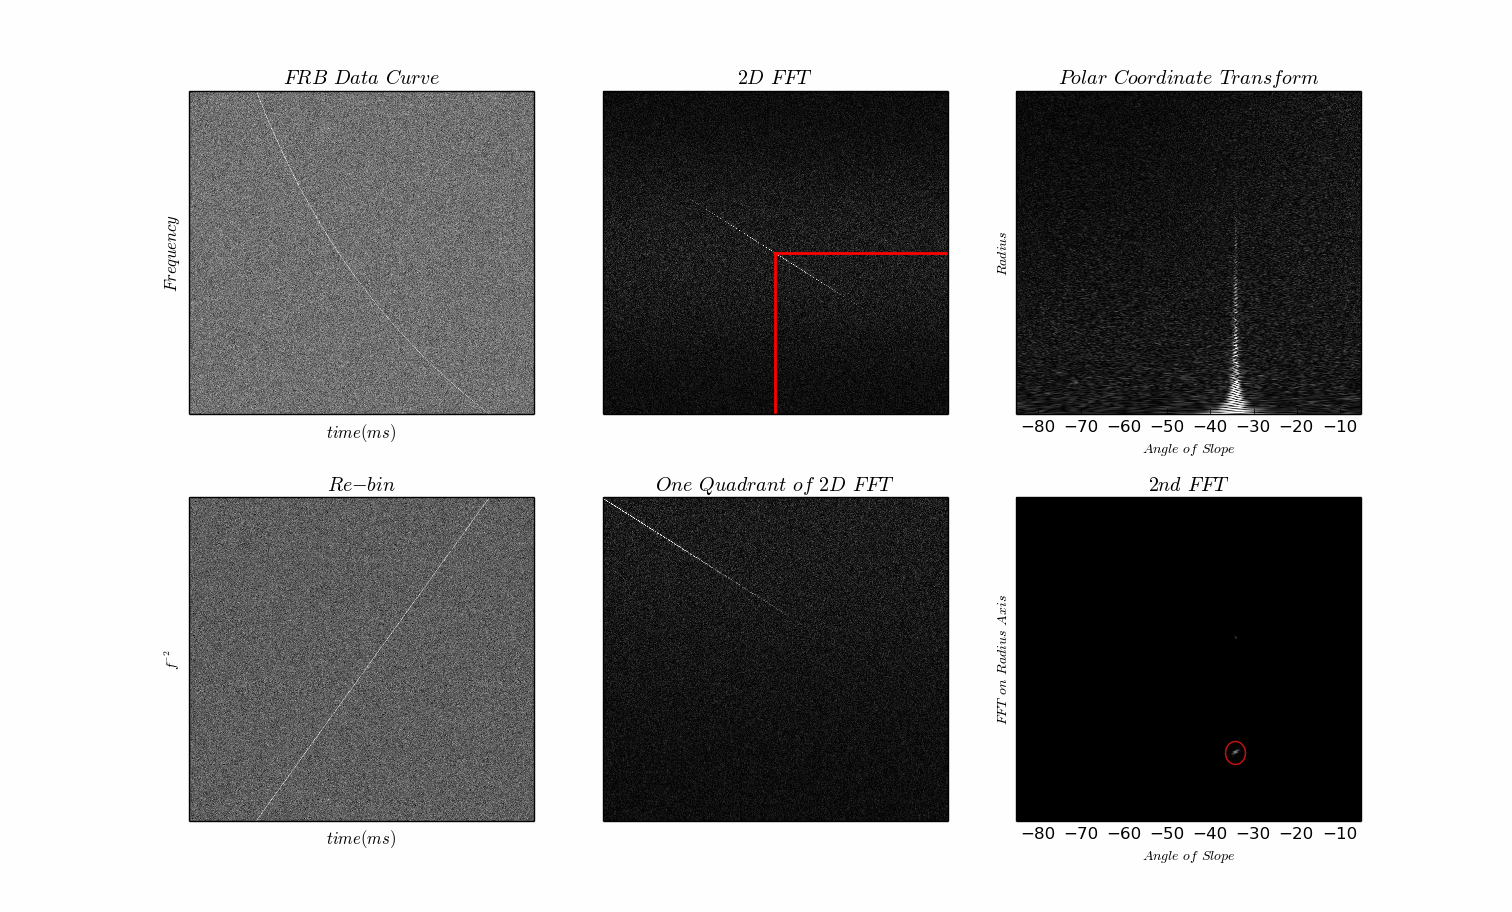
\includegraphics[width=180mm]{./pictures/procedure1.png}
\caption{The whole process of 2DFFT algorithm. Left top is Raw data of FRB data curve in $f(t)$ form which are follow Eq(\ref{eq:Disperse relation}). Left bottom is Re-bin process on Raw data,after this process curve in the Left top will comes to a straight line in $f^{-2}(t)$ form. Mid top is Re-bin Data after 2D FFT. Straight line in Left bottom turn into a straigt line that rotate 90$^{\circ}$ and go through center. As discussed in Sec \ref{sec:polar coordinate transform}, we could only take one quadrant data. Here we take data inside red line area of Mid top. One quadrant data are showed in Mid bottom. In Mid bottom image, Left top point is taken as origin and top horizontal line as origin axis, Then calculate the radius and angle of slope of each pixel and change this image into polar coordinate image of $(radius,angle)$ form as showed in Right top. As phase term influence, interference 	texture could be found on 2D FFT image. Then final step is doing 1D FFT along radius axis on polar coordinate data, then entire signal line will converge to several spots as showed in Right bottom.  \label{fig:Procedure}}
\end{figure*}

\subsection{polar coordinate transform}\label{sec:polar coordinate transform}

As DM always bigger than zero, so $k_2$ is always positive. It indicate signal after 2D-FFT is a straight line which will only appear in 1/2 of 2DFFT map. For example, Fig.\ref{fig:2DFFT} shows a signal line location after 2DFFT, it won't show up in quadrant \uppercase\expandafter{\romannumeral2} and  \uppercase\expandafter{\romannumeral4}, but only quadrant \uppercase\expandafter{\romannumeral1} and \uppercase\expandafter{\romannumeral3}. nevertheless quadrant \uppercase\expandafter{\romannumeral1} and \uppercase\expandafter{\romannumeral3} are conjugate to each other, we can only take 1 of them.

\begin{figure}
\epsscale{1}
\plotone{./pictures/1stFFT.png}
\caption{Signal on 2DFFT map \label{fig:2DFFT}}
\end{figure}

For purpose of search transient on 2D-FFT map, we need trace every slope of line which go cross center. It's easier to get each straight which pass through center from raius and angle of slope space $(r,\theta)$. Thus it's better to take a coordinate transform.  In Fig. \ref{fig:2DFFT},  If we make use of quadrant \uppercase\expandafter{\romannumeral1}, we can take map center as origin $O$, and horizontal axis as original axis, then each line go cross center will have radius and angle information. 

%It's not necessary to take the whole quadrant \uppercase\expandafter{\romannumeral1}, like the yellow part can be cast off. Because signal line go through 2DFFT will be not that long. Data after 2DFFT are in shape of square, $[N_{ch},N_t]$ for example, we can take the radius as ${\min(N_{ch}/2,N_t/2)}$ when we do polar coordinate transform. There are a lot of ways to take polar coordinate transform. But here we are taking interpolation which might be more smooth. After polar coordinate transform, signal line will exist at some exact angle $\theta$. As shows in right top of Fig \ref{fig:Procedure}. 

As tiny scale before FFT will decide large structure after FFT. Taking care of direction of FFT, Signal length in 2D-FFT map depend on width of signal line on re-bin map. Similarly, For polarization coordinates transform, the angle resolution could get from the length of signal line on re-bin map.  Note width and length of signal before 2D-FFT is $w_s$ and $l_s$, the length and width of signal after 2D-FFT will be $l_{FFT}=1/w_s$ and $w_{FFT}=1/l_s$ separately. Dimension of pixel need to be considered when actually process.
Thus It's not necessary to take the whole data of quadrant \uppercase\expandafter{\romannumeral1} but pixels whose radius value smaller tan $l_{FFT}$.  Furthermore, if $DM$ range are already set up, the boundary angle of slope $[\theta_{DM_{min}},\theta_{DM_{max}}]$ are also been decided according to Eq \ref{seq:DM Calculate}.  Thus pixel whose angle of slope are beyond boundary could be cast through.
%Actually,  if DM range is given, only small part of data are useful and 
%Because length of signal after 2D-FFT will be shortened.  That Data after 2DFFT are in shape of square, $[N_{ch},N_t]$ for example, we can take the radius as ${\min(N_{ch}/2,N_t/2)}$ when we do polar coordinate transform. 

There are a lot of ways to take polar coordinate transform. But here we are taking interpolation which might be more smooth. 
%Interpolation algorithm are showed on Algorithm I.
%\begin{algorithm}[H]
%\caption{The Interpolation Algorithm}
%\label{interpolation}
%Input: Data after FFT denote in $\mathcal{F}(f^{-2},t)$ whose shape assume to be $[N_{chan}, N_{samp}]$; $DM$ range that observer want to search; Reasonable width of pulse:$w_s$, Generally take minimum width                                                 value from FRB already known. 
%
%Output: Polar coordinate data denote in $\mathcal{P}(r,\theta)$. Shape of data is $[N_r,N_{\theta}]$.
%
%\begin{algorithmic}
%  %\scriptsize
%  \STATE Calculate $\theta$ boundary and $r$ range from given 
%  
%  \FOR{iteration $i=1$ to $i=log_2{N_f}$}
%  \FOR{$f_0$ in the range $\left[f_{\min},f_{\max}\right]$ with steps $2^i\delta_f$}
%   
%  \STATE $f_2 = f_0 + 2^i\delta_f$
%  \STATE $f_1 = \frac{f_2 - f_0}{2}$
%  \STATE $C_{f_2,f_0} = \frac{f_1^{-2} - f_0^{-2}}{f_2^{-2} - f_0^{-2}}$
%  \STATE $\Delta t_{\max}(i,f_0) = N_\Delta \frac{f_0^{-2} - (f_0 + 2^i\delta_f)^{-2}} {f_{\min}^{-2} - f_{\max}^{-2}} $
%  \FOR{$\Delta t$ in the range $[0,\Delta t_{\max}(i,f_0)]$}
%  \FOR{$t_0$ in range $[C_{f_2,f_0} \Delta t,N_t]$}
%  \STATE $t_1 = t_0 - C_{f_2,f_0}\Delta t$
%  \STATE
%  $
%  A_{f_0}^{f_2}(t_0,\Delta t) = A_{f_0}^{f_1}(t_0,t_0-t_1) + A_{f_1}^{f_2}(t_1,t_1-t_2)
%  $
%  \ENDFOR
%  \FOR{$t_0$ in the range $[0,C_{f_2,f_0} \Delta t]$}
%    \STATE
%    $
%    A_{f_0}^{f_2}(t_0,\Delta t) = A_{f_0}^{f_1}(t_0,C_{f_2,f_0} \Delta t)
%    $
%    \ENDFOR
%    
%  
%  \ENDFOR
%  \ENDFOR 
%  \ENDFOR
%  
%\end{algorithmic}
%\end{algorithm}

 After polar coordinate transform, signal line will exist at some exact angle $\theta$. As shows in right top of Fig \ref{fig:Procedure}. 

\subsection{Turn signal line into spot}
As we discussed before, the phase term $e^{-i2\pi vb}$ could disturb the signal. Since phase term is monotonically and data are complex number, if we integrate along radius directly, signal intensity will be blended. We also can't take absolute value then sum,  due to noise will be amplified. A reasonable method is to take another FFT along radius axis, so that the influence of phase term will be eliminated.
After this we could get Signal Noise Ratio by 
\begin{equation*}
SNR = \frac{Max~Value }{std}
\end{equation*}
When we know where the highest SNR is , we can got the slope of it , finally calculate the DM Value from Eq.(\ref{seq:DM Calculate}). 
The entire procedure are showed by Fig\ref{fig:Procedure} The Data are generated by SIGPROC and parameter are simulated from TianLai Array FRB backend request which Time resolution is 1 millisecond, Band width is 100 MHz and central Frequency is 750 Mhz,  with 1024 Frequency Channels.


\subsection{Advantage on RFI removing}
There are two sorts of regular RFI: At certain frequency last long time, At certain time stamp but with large bandwidth, corresponding to horizontal and vertical line separately in image of Re-bin data. After 2D FFT , they will rotate 90$^{\circ}$, but all of them go through center no matter what frequency or time stamp they are. Therefore, Regular type of RFI could be removed simply by discarding data after 2D FFT at horizontal and vertical line that go cross center.%0$^{\circ}$ and -90$^{\circ}$. 
An example could be seen from Fig. \ref{fig:RFI remove}.

\begin{figure}[ht!]
\centering
\subfigure[Add RFI manually on Re-bin map]{
\epsscale{1.1}
\plotone{./pictures/RFI_remove-1.png}
}
\subfigure[RFI are removed on 2D FFT map]{
\plotone{./pictures/RFI_remove-2.png}}
\caption{Plot (a) shows Re-bin map which are add 3 RFI manully: Time domain and frequency domain and short bad data area. Seeing from Plot (b), RFI are removed clearly.  \label{fig:RFI remove}}
\end{figure}


\section{Detection of observed FRB data}
Observed FRB data are tested through this algorithm. 
%\section{Compute Complexity and benchmark}
\section{Incoherent De-dispersion algorithms and Compute Complexity}
There are a lot of incoherent transient search algorithm already in use, But I'd like to difference them into four types: 1) $Brute~force$ 2) $Tree~algorith$ , 3) $Image~processing$.  

$Brute Force$ is implemented in a lot of software like $SIGPROC$, $HEIMDALL$. In general, the compute complexity of transient search algorithm is compute dependency on number of time samples $'N_t'$, number of frequency channels $'N_{\nu}'$ and number of DM $'N_{DM}'$ of observation. The basics of $Brute Force$ is to shift time delays back for each frequency channel according to Eq\ref{eq:Disperse relation}. As every DM are processed with every time sample and frequency channel, so the total compute complexity is $(N_t N_{\nu} N_{DM})$. It has the slowest compute complexity along the 3 types, However it is easier to paralleliz and implement on GPUs which are good at high performance computing. $HEIMDALL$ is an example to take use GPU to De-disperse. It has been used for a lot of real-time survey like UTMOST \ref{} and ??? and already detected lots of FRB instances. 

Different with $Brute Force$ algorithm, Talor proposed $Tree$ algorithm \ref{} to accelarate $Brute Force$ de-disperse algorithm. Under asumption of Eq \ref{eq:linear assumpution}, Tree algorithm trace signal across a straight line and reuse some element to get rid of redundant calculation. It has same mechanisim as FFT and compute complexity is $(N_t N_{\nu} \log_2{N_{\nu}})$.	Though Tree algorithm is much faster than $Brute Force$, it is difficult at pratical application. The result are iterative at each step, This algorithm has worse  parallelism. As for Linear aproximate, it also face SNR lost. Advanced 'Tree' method are raised up. People are using sub frequency band to get curve more like straigt and also can parallel at that time. Moreover, 'FDMT' are proposed to get accurate curve calculated in decent subband. In 'FDMT' algorithm, the compute complexity is $\max \{N_tN_{DM}\log_2(N_{\nu}),2N_{\nu}N_t\}$.

Algorithm disscuessed in this paper is belong to $Image processing$ way to De-disperse. This type of algorithm foucus on finding a signal line on given $(f,t)$ data. Excpet algorithm talked in this paper, there are a lot of ways to complish this algorithm, like Radnom transform and Machine learning. The compute complexity is varied with different implement method. For 2D-FFT algorithm talked in this papaer, The most time consuming step is 2D-FFT. Though a second 1-D FFT are executed on $(r,\theta)$ data, this doesn't change due to $N_t$,$N_{\nu}$, or $N_{DM}$. Because data shape after polar coordinate transform is only decided by supposed signal width $w_s$ and assumed signal length $l_s$ which are constant during a observation. The scale need to process are much smaller than 2D-FFT . Thus the compute complexity got from this algorithm are mainly caused by 2D-FFT which are $2N_t N_{\nu} \log_2(N_t N_{\nu})$. 

\begin{deluxetable*}{lccc}[H]  % <--- column justification (center/left/right)
\tablecolumns{4}
\tablecaption{Algorithm comparison \label{AlgorithmComparisonTable}}
\tablehead{   % column headings
  \colhead{} &
  \colhead{FDMT} &
  \colhead{Brute force} &
  \colhead{Tree}
}
\startdata
Computational complexity & $\max\{N_tN_{\Delta}\log_2(N_f),2N_fN_t\}$ & $N_fN_tN_{\Delta} $& $N_fN_t\log_2(N_f)$ \\
Information efficient    & Yes & Yes  & No \\
Memory access friendly   & Yes & Yes & Yes \\
Parallelization friendly & Yes & Yes & No \\
\enddata
\tablecomments{Comparison of the FDMT algorithm with two other approaches to incoherent dedispersion, brute force (e.g.,It is clear that the FDMT algorithm dominates in all parameters.}
\end{deluxetable*}


	Table \ref{tabel:1} shows comparation with some Transients search algorithm like $Brute Force$, $Tree$, $FDMT$. This algorithm doesn't have simplest compute complexity.  Take Tree algorithm for example, this method will twice the complexity.  However there are advantages that we might be interested. 

\subsection{Benchmark}
\begin{figure}[ht!]
\epsscale{1}
\plotone{./pictures/benchmark.png}
\caption{Benchmark of Transient search software: Sigproc, Sigpyproc, Heimdall , 2DFFT \label{fig:benchmark}}
\end{figure} 
 
\bibliography{paper}
%\begin{deluxetable*}{lccc}  % <--- column justification (center/left/right)
%\begin{figure}[ht!]
%\epsscale{1.2}
%\plotone{./pictures/procedure1.png}
%\caption{The whole process of 2DFFT algorithm. Left top is Raw data of FRB data curve in $f(t)$ form which are follow Eq(\ref{eq:Disperse relation}). Left bottom is Re-bin process on Raw data,after this process curve in the Left top will comes to a straight line in $f^{-2}(t)$ form. Mid top is Re-bin Data after 2D FFT. Straight line in Left bottom turn into a straigt line that rotate 90$^{\circ}$ and go through center. As discussed in Sec \ref{sec:polar coordinate transform}, we could only take one quadrant data. Here we take data inside red line area of Mid top. One quadrant data are showed in Mid bottom. In Mid bottom image, Left top point is taken as origin and top horizontal line as origin axis, Then calculate the radius and angle of slope of each pixel and change this image into polar coordinate image of $(radius,angle)$ form as showed in Right top. As phase term influence, interference 	texture could be found on 2D FFT image. Then final step is doing 1D FFT along radius axis on polar coordinate data, then entire signal line will converge to several spots as showed in Right bottom.  \label{fig:Procedure}}
%\end{figure}
%\end{deluxetable*}

\begin{thebibliography}{}
\expandafter\ifx\csname natexlab\endcsname\relax\def\natexlab#1{#1}\fi
\providecommand{\url}[1]{\href{#1}{#1}}

\bibitem[{{Alam} {et~al.}(2015){Alam}, {Albareti}, {Allende Prieto}, {Anders},
  {Anderson}, {Anderton}, {Andrews}, {Armengaud}, {Aubourg}, {Bailey}, \&
  et~al.}]{aaa+15}
{Alam}, S., {Albareti}, F.~D., {Allende Prieto}, C., {et~al.} 2015, \apjs, 219,
  12

\end{thebibliography}



\end{document}



%\begin{figure*}
%  \center
%  \includegraphics[width=0.9\textwidth]{nustar_regions}
%  \includegraphics[clip=true,trim=0.3in 0.3in 1.1in 0.8in,width=0.45\textwidth]{backgrounds_A}
%  \includegraphics[clip=true,trim=0.3in 0.3in 1.1in 0.8in,width=0.45\textwidth]{backgrounds_B}
%  \caption{}
%  \label{fig:nustar_regions}
%\end{figure*}


%\begin{deluxetable}{lcccc}
%  \centering
%  \tablecolumns{5} 
%  \tablecaption{X-ray Observations of \igr\ in 2014.\label{tab:obs}}
%  \tablewidth{0pt}
%  \tabletypesize{\footnotesize}
%  \tablehead{
%    \colhead{Obs ID/Rev\tablenotemark{a}}   &
%    \multicolumn{2}{c}{Obs Time (UT)\tablenotemark{b}} & 
%    \colhead{Exp}      &
%    \colhead{Rate}\\
%    \colhead{}  &
%    \colhead{Start}                    &
%    \colhead{End}                    &
%    \colhead{(ks)}                 &
%    \colhead{(cts/s)}
%  }
%  \startdata 
%  \sidehead{\nustar}           %MJD-OBS            TELAPSE  
%  80001046002 & 10-10 08:51:07 & 10-11 00:46:07 & 29.4& 3.5--4  \\  %56940.38413696764  5.562777499043941E+04

%  \sidehead{\integral}
%  1458        & 09-21 19:03:49 & 09-24 04:25:41 & 28.7  & 3.1\\  

% \enddata
%\tablecomments{}
%\tablenotetext{a}{}
%\tablenotetext{b}{}
%\tablenotetext{p}{}
%\end{deluxetable}

%\begin{deluxetable}{clcc}
%  \centering
%  \tablecolumns{4} 
%  \tablecaption{Optical Observations of \frb \label{tab:obs}}
%  \tablewidth{0pt}
%  \tabletypesize{\footnotesize}
%  \tablehead{
%    % Date, Filt/Grating, Exposure, Conditions 
%    \colhead{Date}   &
%    \colhead{Filter/} & 
%    \colhead{Exposure}      &
%    \colhead{Conditions}\\
%    \colhead{UTC}  &
%    \colhead{Grating}  &
%    \colhead{(s)} &
%    \colhead{\texttt{IQ},\texttt{CC},\texttt{WV},\texttt{BG}\tablenotemark{a}}                 
%  }
%  \startdata 
% % \sidehead{\nustar}           %MJD-OBS            TELAPSE  
% % 80001046002 & 10-10 08:51:07 & 10-11 00:46:07 & 29.4& 3.5--4  \\  %56940.38413696764  5.562777499043941E+04
%2016-10-24 & $r^\prime$ & 500 & 20,70,50,50\\
%2016-10-25 & $r^\prime$ & 750 & 70,70,20,20\\
%2016-11-02 & $i^\prime$ & 1200 & 20,50,20,20\\
%2016-11-02 & $z^\prime$ & 1800 & 70,50,20,20\\
%2016-11-09 & R400/675\tablenotemark{b} & 7200 & 20,50,100,20\\
%2016-11-10 & R400/690\tablenotemark{b} & 5400 & 70,50,100,20\\
%2016-11-10 & R400/675\tablenotemark{b} & 3600 & 70,50,100,20\\
% \enddata
%%\tablecomments{}
%\tablenotetext{a}{Image quality (\texttt{IQ}), Cloud Cover (\texttt{CC}), Water Vapor (\texttt{WV}), and Sky Background (\texttt{BG}) conditions in percentiles for the Gemini North Observatory site on Mauna Kea. \texttt{IQ}20 and \texttt{IQ}70 correspond to 0\farcs50 and 0\farcs75 zenith seeing in $i^\prime$ band, respectively. \texttt{BG}20 and \texttt{BG}50 correspond to sky surface brightness of $\upmu_V > 21.3\,\mathrm{mag\,arcsec^{-2}}$ and $ > 20.7\,\mathrm{mag\,arcsec^{-2}}$, respectively. }
%\tablenotetext{b}{Grating and central wavelength in nm.}
%\end{deluxetable}


